\documentclass[letterpaper, 12pt]{article}

\usepackage[english]{babel}
\usepackage[margin=0.85in]{geometry}
\usepackage{graphicx}
\usepackage{float}
\usepackage{subcaption}
\usepackage{hyperref}
\newenvironment{allintypewriter}{\ttfamily}{\par}
\hypersetup{
  colorlinks,
  citecolor=black,
  filecolor=black,
  linkcolor=black,
  urlcolor=black
}

\date{}
\graphicspath{{quickstartpics/}}
\newcommand\TSAT{\textbf{TSAT}}

\begin{document}
\title{TSAT Quickstart Guide}
\maketitle
\noindent
Time Series Analysis Tool, \TSAT, has three main features:
\begin{description}
	\item[Supervised Classification] Using labeled time series train an algorithm to classify unknown
	\item[Motif Discovery] Finding repeated patterns within a time series
	\item[Anomaly Detection] Finding rarely repeated patterns within a time series
\end{description}
Here we will use \textbf{supervised classification} to determine the accuracy on a test dataset.

\section{Load Dataset and Train Classifier}
\vspace{-.6em}
\begin{figure}[H]
	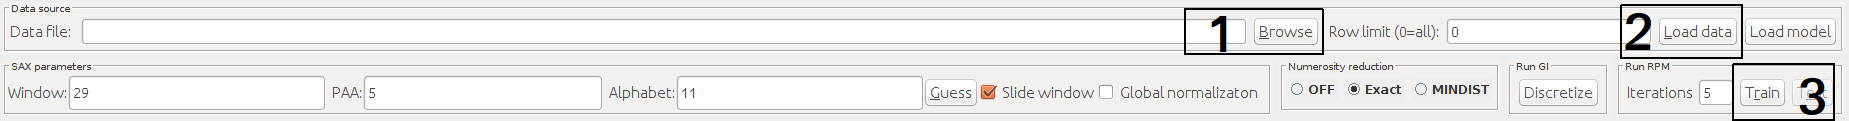
\includegraphics[width=\textwidth]{quickstartpics/trainfull}
	\textbf{1} Click ``Browse'' and navigate to your training dataset.\\ \textbf{2} Click ``Load data'' which will also display the time series in data display area.\\ \textbf{3} Click ``Train'' to train the classifier on the training data.  When training is done the text area will display: \texttt{view: RPM Handler: Finished RPM Training in Background}
	\label{fig:browseload}
\end{figure}

\section{Test the Classifier}
\vspace{-.6em}
\begin{figure}[H]
	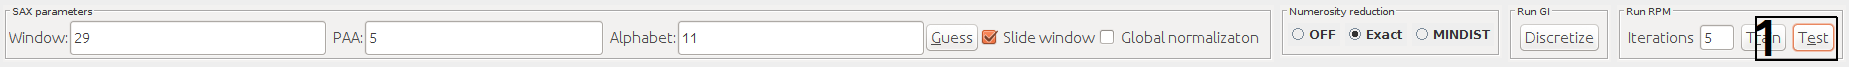
\includegraphics[width=\textwidth]{quickstartpics/test}
	 \textbf{1} Click ``Test'' to load the test data and start testing to determine the accuracy of the classifier.
	 \\When testing is done the text area will show: \texttt{model: Finished testing see tabs labeled RPM Classification and RPM Time Series Results for result info}
	\label{fig:test}
\end{figure}

\section{Test Results}
\vspace{-.6em}
\begin{figure}[H]
	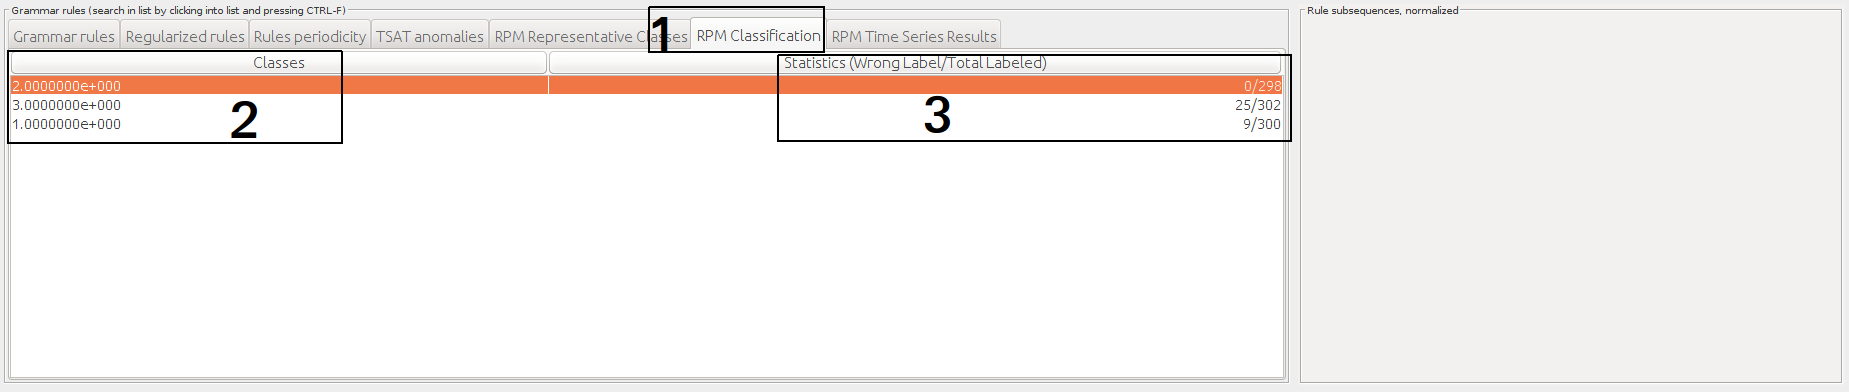
\includegraphics[width=\textwidth]{quickstartpics/testresults}
	\textbf{1} Click on the ``RPM Classification'' tab to view the accuracy results.\\ \textbf{2} Classes column contains the labels.\\ \textbf{3} Statistics column contains the number of misclassified examples for each class.
	\label{fig:testresults}
\end{figure}


\end{document}
